\documentclass[12pt, twoside]{article}
\usepackage[letterpaper, margin=1in, headsep=0.2in]{geometry}
\setlength{\headheight}{0.6in}
%\usepackage[english]{babel}
\usepackage[utf8]{inputenc}
\usepackage{microtype}
\usepackage{amsmath}
\usepackage{amssymb}
%\usepackage{amsfonts}
\usepackage{siunitx} %units in math. eg 20\milli\meter
\usepackage{yhmath} % for arcs, overparenth command
\usepackage{tikz} %graphics
\usetikzlibrary{quotes, angles}
\usepackage{graphicx} %consider setting \graphicspath{{images/}}
\usepackage{parskip} %no paragraph indent
\usepackage{enumitem}
\usepackage{multicol}
\usepackage{venndiagram}

\usepackage{fancyhdr}
\pagestyle{fancy}
\fancyhf{}
\renewcommand{\headrulewidth}{0pt} % disable the underline of the header
\raggedbottom
\hfuzz=2mm %suppresses overfull box warnings

\usepackage{hyperref}

\fancyhead[LE]{\thepage}
\fancyhead[RO]{\thepage \\ Name: \hspace{4cm} \,\\}
\fancyhead[LO]{BECA / Dr. Huson / Geometry\\*  Unit 2: Angles\\* 6 October 2022}

\begin{document}

\subsubsection*{2.7 Test: Extension topics}
\emph{Diagrams are not necessarily drawn to scale unless otherwise stated.}
\begin{enumerate}

\item The protractor shown below is marked with degree measures on the inside and radian measures on the outside. Make a 1 radian angle by drawing a ray from the center $V$ through the protractor semicircle. \par \medskip
  \begin{center}
  \begin{tikzpicture}
    \draw[thick] (-3,0)--(0,0)--(3,0);
    \draw (4,0) arc (0:180:4);
    \fill (0,0) circle [radius=0.05]node[below]{$V$};
    \foreach \x in {0,15,30,...,180}
      \node at (\x:3.4){\x};
    \foreach \x in {0,15,30,...,180}
      \draw (\x:3.7)--(\x:4);
    \foreach \x in {0,5,...,180}
      \draw (\x:3.9)--(\x:4);
    \foreach \x in {0,0.1,...,3.1}
      \draw (57.3*\x:4)--(57.3*\x:4.3);
    \foreach \x in {0.2,0.4,0.6,0.8,1.0,1.2,1.4,1.6,1.8,2.0,2.2,2.4,2.6,2.8,3.0}
      \node at (57.3*\x:4.7){\x};
    \draw (-4.3,0)node[left]{$\pi$}--(-4,0);
    \draw[->,thick] (4,0)--(0:6);
    \end{tikzpicture}
  \end{center}

\item Use the protractor above to convert radians and degrees. (nearest whole degree, nearest hundredth radian).
  \begin{multicols}{2}
    \begin{enumerate}
      \item $80^\circ = $ \vspace{0.7cm}
      \item $28^\circ = $ \vspace{0.7cm}
      \item $\displaystyle 1.0 \text{ radian} =$ \vspace{0.7cm}
      \item $\displaystyle 2.7 \text{ radian} =$
    \end{enumerate}
  \end{multicols}

\item Given $x=-3$ simplify each expression. (try to do them without a calculator)
  \begin{multicols}{2}
    \begin{enumerate}[itemsep=1.25cm]
      \item $|x-1|=$
      \item $2 \times|x+2|=$
    \end{enumerate}
  \end{multicols} \vspace{1cm}

\item Find all values of $x$ satisfying the equation. (show the two cases and checks) 
  $$ |x+2|+7 = 17$$

\newpage
\item Convert each value to scientific notation.
  \begin{multicols}{2}
    \begin{enumerate}[itemsep=1cm]
      \item 70,000 =
      \item 860,000 =
    \end{enumerate}
  \end{multicols} \vspace{1cm}

\item Expand each value to regular numeric form. (i.e. an integer)
  \begin{multicols}{2}
    \begin{enumerate}[itemsep=1cm]
      \item $3 \times 10^{6}=$
      \item $1.25 \times 10^{3}=$
    \end{enumerate}
  \end{multicols} \vspace{0.7cm}

\item Round each value to the \emph{nearest hundredth}.
  \begin{multicols}{2}
    \begin{enumerate}
      \item $1 \text{ radian}=57.29577951...^\circ$ \par 
      \item $\sqrt{5} \approx$
    \end{enumerate}
  \end{multicols} \smallskip 

\item Round each value to the nearest thousand.
  \begin{multicols}{2}
    \begin{enumerate}
      \item $53,997 \approx$ \par \bigskip (the area of Florida in square miles)
      \item $42,224 \approx$ \par \bigskip (the area of New York)
    \end{enumerate}
  \end{multicols}

\item The distance in miles from New York City to Santo Domingo, Dominican Republic is 1,554 miles. Convert that distance to kilometers. (1 mile $\approx$ 1.61 kilometers) \vspace{2cm}

\emph{Use the formula for percent error in the following problem}
$$\epsilon = \left|\frac{v_A-v_E}{v_E}\right| \times 100\%$$

\item The actual length of earth's year is about 365.25 days. Find the percent error of using an approximation of 360 days.

\newpage
\item In the diagram below $\angle BOC = 7x-50$ and $\angle DOE = 4x-3$. Find m$\angle AOB$. \vspace{0.25cm}
\begin{flushright}
\begin{tikzpicture}[scale=1.3, rotate=-20]
  \draw[<->, thick] (-40:3)--(0,0)--(140:3);
  \draw[<->, thick] (-3,0)--(3,0);
  \draw[->, thick] (0,0)--(0,3);
  \draw (0,0)++(0.3,0)--++(0,0.3)--+(-0.3,0);
  \draw[fill] (140:2) circle [radius=0.05] node[below left]{$B$};
  \draw[fill] (-2,0) circle [radius=0.05] node[below]{$A$}; 
  \draw[fill] (0,0) circle [radius=0.05] node[below left]{$O$};
  \draw[fill] (0,2) circle [radius=0.05] node[left]{$C$};
  \draw[fill] (2,0) circle [radius=0.05] node[below]{$D$};
  \draw[fill] (-40:2) circle [radius=0.05] node[left]{$E$};
\end{tikzpicture}
\end{flushright} \vspace{1cm}

\item In the diagram below $\angle AOB = x-7$ and $\displaystyle \angle COD = \frac{3}{4}(x+57)$. Find $\angle BOC$ \vspace{0.25cm}
\begin{flushright}
\begin{tikzpicture}[scale=1, rotate=0]
\draw[->, thick] (0,0)--(155:5);
\draw[<->, thick] (-5,0)--(5,0);
\draw[->, thick] (0,0)--(0,4);
\draw (0,0)++(0.3,0)--++(0,0.3)--+(-0.3,0);
\draw[fill] (155:3) circle [radius=0.05] node[below left]{$B$};
\draw[fill] (-4,0) circle [radius=0.05] node[below]{$A$}; 
\draw[fill] (0,0) circle [radius=0.05] node[below]{$O$};
\draw[fill] (0,3) circle [radius=0.05] node[left]{$C$};
\draw[fill] (4,0) circle [radius=0.05] node[below]{$D$};
\end{tikzpicture}
\end{flushright}

\newpage
\item In the line segment $\overline{ABC}$, $\overline{AB}$ is twice as long as $\overline{BC}$. $AB=12x-6$ and $AC=15x+9$. Find $BC$.
\vspace{5cm}

\item Mark the positions of the minute and hour hands at 4:00. Write down the measure in degrees of the angle made by the two clock hands. \par \vspace{0.25cm}
  \begin{tikzpicture}
    \draw (0,0) circle [radius=2];
    \draw (0,0) circle [radius=0.1];
    \foreach \x in {1,...,12}
      \node at ({90+\x*-30}:1.8){\x};
  \end{tikzpicture}

\item A compound shape composed of two rectangles is shown with dimensions marked, both having heights of 6 cm and with base lengths of 2 cm and 5 cm respectively.
  \begin{multicols}{2}
    \begin{tikzpicture}
      \draw[thick] (0,0) rectangle (6,5);
      \draw[thick] (2,0) -- (2,5);
      \node at (6.5,3){6};
      \node at (1,-0.4){2};
      \node at (4,-0.4){5};
    \end{tikzpicture}
    \begin{enumerate}
      \item Find the perimeter of the smaller rectangle on the left. \vspace{2cm}
      \item Find the total area of the combined rectangles
      \end{enumerate}
    \end{multicols} \vspace{1cm}

\end{enumerate}
\end{document}